\documentclass{beamer}
\usepackage{amsmath}
\usepackage{subfig}
\usepackage[backend=biber, style=authoryear]{biblatex}
\addbibresource{references.bib}
\usetheme{Antibes}
\title{Improving sequantial recommendation model with MSE}
\author{Noora Pöysti \& Väinö-Waltteri Granat}

\begin{document}
\frame{\titlepage}


\begin{frame}
    \frametitle{Basic idea}
    We want to improve the calculation of $\alpha_{j}$ by taking all the users satisfactions in to account while
    giving more weight to the least satisfied users. We can achieve this with MSE.
\end{frame}

\begin{frame}
    \frametitle{Improved $\alpha_j$}

    $\alpha_j$ is calculated with MSE (mean squared error) but instead of using a square we take cube root of the square
    to allow $\alpha_j$ to increase in value when dissatisfaction is high.

    \begin{align*}
    \alpha_j = \frac{1}{|G|} \sum_{u\in G} \sqrt[3]{(max_{u'\in G} sat(u',Gr_{j-1}) - sat(u, Gr_{j-1}))^2}
    \end{align*}

    MSE exaturates the error when distance between values is high, so the algorithm will but more weight for the iterations 
    when lots of disagreement is present.
\end{frame}

\begin{frame}
    \frametitle{Comparison}
    \begin{figure}%
        \centering
        \subfloat[\centering original]{{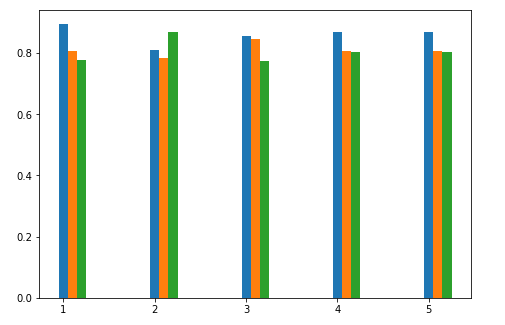
\includegraphics[width=0.45\textwidth]{original_alpha.PNG} }}%
        \qquad
        \subfloat[\centering with MSE]{{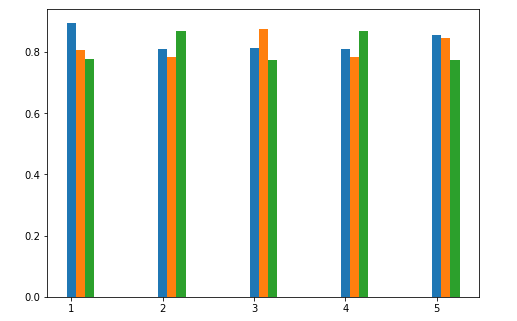
\includegraphics[width=0.45\textwidth]{improved_alpha.PNG} }}%
        \caption{Comparison between original $\alpha_j$ and $\alpha_j$ calculated with MSE}%
        \label{fig:example}%
    \end{figure}
\end{frame}
\end{document}
